\documentclass[30pt,twocolumn,letterpaper]{article}
\usepackage{cvpr}
\usepackage{times}
\usepackage{booktabs}
\usepackage{epsfig}
\usepackage{graphicx}
\usepackage{amsmath}
\usepackage{amssymb}
\cvprfinalcopy
\def\cvprPaperID{****}
\def\httilde{\mbox{\tt\raisebox{-.5ex}{\symbol{126}}}}
\usepackage{graphicx}
\usepackage{indentfirst}
\setlength{\parindent}{2em}
\usepackage{cite}
\usepackage[colorlinks,linkcolor=red,anchorcolor=blue,citecolor=green,backref=page]{hyperref}
\author{Qilei Zhang\\\\
Jun 8 2018}
\title{Deep Learning of Representations for Unsupervised and Transfer Learning}
\begin{document}
\maketitle
\begin{abstract}
  Deep learning algorithms seek to exploit the unknown structure in the input distribution in order to discover good representations, often at multiple levels, with higher-level learned features defined in terms of lower-level features.
\end{abstract}
\section{Introduction}
The objective is to make these higherlevel representations more abstract, with their individual features more invariant to most of the variations that are typically present in the training distribution, while collectively preserving as much as possible of the information in the input. Machine learning algorithms attempt to discover structure in data. In their simpler forms, that often means discovering a predictive relationship between variables. More generally,that means discovering where probability mass concentrates in the joint distribution of all the observations\cite{Baldi2014Searching}. \\
\begin{figure}[htbp]
\small
\centering
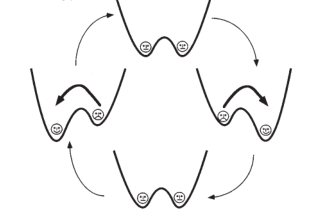
\includegraphics[width=20em]{000.png}
\caption{Transfer ratios on the Amazon benchmark. Both SDA-based systems outperforms the rest, and SDAsh (unsupervised training on all domains) is best.Reproduced from Glorot et al. (2011b).}
\label{fig:lable}
\end{figure}\\
\par
Many researchers have found that the way in which data are represented can make a huge difference in the success of a learning algorithm. \cite{Lenz2013Deep}.
\begin{equation}
\quad x'=f(x)+A_0cos(wt+o)+u(t)
\end{equation}

\section{The Context of The Unsupervised and Transfer Learning Challenge}
The challenge was organized according to the following learning setup. The test sets have examples from classes not well represented in the training set. They have only a small number of unlabeled examples and very few labeled examples available to a Hebbian linear classifier  applied separately to each class against the others\cite{Warburton2003Deep}. \\
{\small
\bibliographystyle{ieee}
\bibliography{1}
}
\end{document}
